\section[一维谐振子]{一维谐振子} \label{sec:02.05} % 
% \makebox[5em][s]{} % 短题目拉间距

设质量为$m$的粒子受到弹性力$F=-kx$作用,则势能为
\begin{empheq}{equation*}
	V(x)=\int_{0}^{x} F(x)dx=\frac{1}{2}kx^{2}
\end{empheq}
令$k=m\omega^{2}$,$\omega>0$,$V(x)$可以写成
\begin{empheq}{equation}\label{eq25.1}
	V(x)=\frac{1}{2}m\omega^{2}x^{2}
\end{empheq}
在这势场作用下,粒子的经典力学运动为谐振动,即
\begin{equation}\label{eq25.2}
	\begin{aligned}
		x(t)&= A\sin(\omega t+\alpha)\quad \text{(A为振幅)}	\\
		v(t)&=\frac{dx}{dt}=\omega A\cos(\omega t+\alpha)
	\end{aligned}
\end{equation}
总能为
\begin{empheq}{equation}\label{eq25.3}
	E=T+V=\frac{m}{2}(v^{2}+\omega^{2}x^{2})=\frac{1}{2}m\omega^{2}A^{2}
\end{empheq}
谐振动可以作为许多实际问题的近似模型,例如粒子在平衡位置[$V(x)$取极小处]附近的小振动可以近似表示成谐振动.电磁场的振动可以分解成各种频率的谐振动,带电粒子在均匀磁场中作圆周运动可以看成两个方向互相垂直的谐振动,等等.

量子力学中,一维谐振子是指在势场\eqref{eq25.1}中运动的粒子.哈密顿算符为
\begin{empheq}{equation}\label{eq25.4}
	\hat{H}=\hat{T}+V=-\frac{\hbar^{2}}{2m}\frac{d^{2}}{dx^{2}}+\frac{1}{2}m\omega^{2}x^{2}
\end{empheq}
因此定态薛定谔方程是
\setlength{\mathindent}{5em}
\begin{empheq}{equation}\label{eq25.5}
	(\hat{H}-E)\varPsi=\bigg(-\frac{\hbar^{2}}{2m}\frac{d^{2}}{dx^{2}}+\frac{1}{2}m\omega^{2}x^{2}-E\bigg)\varPsi=0
\end{empheq}
由于$x\rightarrow\pm\infty$处$V\rightarrow\infty$,$\varPsi$必须迅速趋于0,这样才能保证$V(x)$的平均值有限.由\eqref{eq23.9}式,势能平均值公式是
\begin{empheq}{equation}\label{eq25.6}
	\bar{V}=\int_{-\infty}^{\infty}V(x)|\varPsi(x)|^{2}dx=\frac{1}{2}m\omega^{2}\int_{-\infty}^{\infty}|x\varPsi(x)|^{2}dx
\end{empheq}\eqnormal
因此$x\varPsi$是平方可积的.这条件比“$\varPsi$平方可积”更为苛刻,也就是说,能使上式为有限值的$\varPsi$必定是平方可积的.因此,谐振子的每一个能量本征态都是束缚态.

\eqref{eq25.5}式中包含三个参量:$\hbar,m,\omega$,它们的量纲互相独立.能量和长度的特征构造应由$\hbar,m,\omega$决定,以$x_{0}$表示特征长度,显然应有
\begin{empheq}{equation*}
	\hbar / mx_{0}^{2}\sim m\omega^{2}x_{0}^{2},\quad x_{0}^{2}\sim\hbar / m\omega
\end{empheq}
\begin{empheq}{equation*}
	E\sim\frac{\hbar^{2}}{mx_{0}^{2}}\sim m\omega^{2}x_{0}^{2}\sim \hbar\omega
\end{empheq}
令
\setlength{\mathindent}{5em}
\begin{empheq}{equation}\label{eq25.7}
	x_{0}=\sqrt{\frac{\hbar}{m\omega}},\quad \alpha=\frac{1}{x_{0}}=\sqrt{\frac{m\omega}{\hbar}},\quad \lambda=\frac{2E}{\hbar\omega}
\end{empheq}\eqnormal
\begin{empheq}{equation}\label{eq25.8}
	\xi=\alpha x=\frac{x}{x_{0}}=\sqrt{\frac{m\omega}{\hbar}}x
\end{empheq}
\eqref{eq25.4}式和\eqref{eq25.5}式可以表示成
\begin{empheq}{equation*}\label{eq25.4'}
	\hat{H}=\frac{\hbar\omega}{2}\bigg(\xi^{2}-\frac{d^{2}}{d\xi^{2}}\bigg)	\tag{$2.5.4^{\prime}$}
\end{empheq}
\begin{empheq}{equation*}\label{eq25.5'}
	\frac{d^{2}}{d\xi^{2}}\varPsi+(\lambda-\xi^{2})\varPsi=0	\tag{$2.5.5^{\prime}$}
\end{empheq}
$\xi$是以$x_{0}$为单位的坐标,$\lambda$是以$\frac{\hbar\omega}{2}$为单位的能量.

$\xi\rightarrow \pm\infty$处,\eqref{eq25.5'}式近似成为
\setlength{\mathindent}{11em}
\begin{empheq}{equation*}
	\frac{d^{2}}{d\xi^{2}}\varPsi\approx\xi^{2}\varPsi
\end{empheq}
其渐近解为
\begin{empheq}{equation*}
	\varPsi\sim e^{\xi^{2}/2},\quad e^{-\xi^{2}/2}
\end{empheq}\eqnormal
由于无限远处$\varPsi$必须趋于0,$\varPsi$的渐近行为应该取$e^{-\xi^{2}/2}$的形式.基于这种理解,令
\begin{empheq}{equation}\label{eq25.9}
	\varPsi=u(\xi)e^{-\xi^{2}/2}
\end{empheq}
代入\eqref{eq25.5'}式,得到$u(\xi)$满足的方程为
\begin{empheq}{equation}\label{eq25.10}
	u^{\prime\prime}-2\xi u^{\prime}+(\lambda-1)u=0
\end{empheq}
$\lambda=\frac{2E}{\hbar\omega}$为待定参数.上式的某些简单特征解可以直接观察出来,例如
\begin{empheq}{align*}
	&u=1,\quad\lambda=1,\quad E\approx\frac{\hbar\omega}{2} \\
	&u=\xi,\quad\lambda=3,\quad E=\frac{3\hbar\omega}{2}
\end{empheq}
$\xi=0$是\eqref{eq25.10}式的正常点,$\xi\rightarrow\pm\infty$则是\eqref{eq25.10}式的唯一奇点.按照微分方程理论,$u(\xi)$必定可以表示成$\xi$的正幕级数:
\begin{empheq}{equation}\label{eq25.11}
	u(\xi)=\sum_{v=0}^{\infty} a_{v}\xi^{v}
\end{empheq}
由于$V(x)$为偶宇称,按照$\S$\ref{sec:02.03}关于束缚态的定理\eqref{eq23.4},\eqref{eq23.5},$\varPsi$应该是具有明确宇称的实函数,而由\eqref{eq25.9}式可知,$u$和$\varPsi$宇称相同,由此可见\eqref{eq25.11}式应该由纯偶次项或纯奇次项构成,即
\setlength{\mathindent}{5em}
\begin{equation*}\label{eq25.11'}
	u(\xi)=
	\begin{cases}
		a_{0}+_{2}\xi^{2}+a_{4}\xi^{4}+\cdots\quad\text{(偶宇称)}	\\
		a_{1}\xi+a_{3}\xi^{3}+a_{5}\xi^{5}+\cdots\text{(奇宇称)}	\tag{$2.5.11^{\prime}$}	
	\end{cases}
\end{equation*}\eqnormal
将\eqref{eq25.11}式代入\eqref{eq25.10}式,比较$\xi$同幕次项系数,容易得到
\begin{empheq}{equation}\label{eq25.12}
	a_{v+2}=\frac{a_{v}(2v+1-\lambda)}{(v+1)(v+2)}
\end{empheq}
利用这个递推公式,就可以将\eqref{eq25.11'}式中全部系数算出.($a_{0}$或$a_{1}$作为归一化系数对待.)

由\eqref{eq25.12}式容易看出,对于偶宇称态,如$\lambda=1$,则$a_{2}=_{4}=\cdots=0$;对于奇宇称态, 如$\lambda=3$,则$a_{3}=a_{5}=\cdots=0,u=a_{1}\xi$.这正是上面指出的两种简单特征解.推广来说,如
\begin{empheq}{equation}\label{eq25.13}
	\lambda=2n+1,\quad n=0,1,2,\cdots
\end{empheq}

\begin{empheq}{equation}\label{eq25.14}
	E_{n}=\frac{\lambda}{2}\hbar\omega=\bigg(n+\frac{1}{2}\bigg)\hbar\omega,\quad n=0,1,2,\cdots
\end{empheq}
这就是谐振子的量子化能级.

如果$\lambda$的值不同于\eqref{eq25.13}式,则任何$a_{v}$都不会等于0,$u(\xi)$表现为无穷级数,这时$u(\xi)$的渐近行为和$e^{\xi^{2}}$相近.理由如下

无穷级数的渐近行为取决于高幕次项.\eqref{eq25.12}式中当$v$很大($v\gg\lambda$)时,
\begin{empheq}{equation*}
	\frac{a_{v+2}}{a_{v}}\approx \frac{2}{v}
\end{empheq}
另一方面,
\begin{empheq}{equation*}
	e^{\xi^{2}}=\sum_{n=0}^{\infty}C_{2n}\xi^{2n}=\sum_{n=0}^{\infty}\frac{\xi^{2n}}{n!},\quad C_{2n}=\frac{1}{n!}
\end{empheq}
\begin{empheq}{equation*}
	\frac{C_{2n+2}}{C_{2n}}=\frac{n!}{(n+1)!}=\frac{1}{(n+1)}
\end{empheq}
即
\begin{empheq}{equation*}
	\frac{C_{v+2}}{C_{v}}=\frac{2}{(v+2)}\quad (v=2n)
\end{empheq}
$v\rightarrow\infty$时,
\begin{empheq}{equation*}
	\frac{a_{v+2}}{a_{v}}\approx\frac{C_{v+2}}{C_{v}}
\end{empheq}
所以$u(\xi)$的渐近行为和$e^{\xi^{2}}$相近.这样,$\varPsi$的渐近行为就是
\begin{empheq}{equation*}
	\varPsi=u(\xi)e^{-\xi^{2}/2}\sim e^{\xi^{2}}e^{-\xi^{2}/2}=e^{-\xi^{2}/2}
\end{empheq}
当$\xi\rightarrow\pm\infty,\varPsi\rightarrow\infty$,不满足波函数的基本要求,不能代表真实状态.

总起来说,谐振子的束缚态能级由\eqref{eq25.14}式表示,波函数由\eqref{eq25.9}式表示,其中$u(\xi)$是$n$次多项式,满足\eqref{eq25.10}式,即
\setlength{\mathindent}{6em}
\begin{empheq}{equation*}\label{eq25.10'}
	u^{\prime\prime}-2\xi u^{\prime}+2nu=0,\quad n=0,1,2,\cdots	\tag{$2.5.10^{\prime}$}
\end{empheq}
称为厄密(Hermite)方程,它的两个独立解中有一个是$n$次多项式,习惯上称为厄密多项式,记为$H_{n}(\xi)$.它的数学性质见附录\ref{A02}.

和能级互相应的归一化波函数记为$\varPsi_{n}$,根据上述,
\begin{empheq}{equation}\label{eq25.15}
	\varPsi_{n}=N_{n}H_{n}(\xi)e^{-\xi^{2}/2}=N_{n}H_{n}\bigg(\frac{x}{x_{0}}\bigg)e^{-x^{2}/2x_{0}^{2}}
\end{empheq}\eqnormal
其中
\begin{empheq}{equation}\label{eq25.16}
	H_{n}(\xi)=(-1)^{n}e^{\xi^{2}}\bigg(\frac{d}{d\xi}\bigg)^{n}e^{-\xi^{2}}
\end{empheq}
\begin{empheq}{equation}\label{eq25.17}
	N_{n}=(x_{0}\sqrt{\pi}2^{n}n!)^{-\frac{1}{2}}
\end{empheq}
\eqref{eq25.16}、\eqref{eq25.17}式的证明见附录\ref{A02}.前几个$H_{n}$利用\eqref{eq25.12}式即可写出.结果得到
\begin{equation}\label{eq25.18}
	\begin{aligned}
		\varPsi_{0}&=(x_{0}\sqrt{\pi})^{-\frac{1}{2}}e^{-x^{2}/2x_{0}^{2}}	\\
		\varPsi_{1}&=\big[x_{0}\frac{\sqrt{\pi}}{2}\big]^{-\frac{1}{2}} \frac{x}{x_{0}}e^{-x^{2}/2x_{0}^{2}}	\\
		\varPsi_{2}&=(2x_{0}\sqrt{\pi})^{-\frac{1}{2}}\bigg(\frac{2x^{2}}{x_{0}^{2}}-1\bigg)e^{-x^{2}/2x_{0}^{2}}
	\end{aligned}
\end{equation}
$\varPsi_{n}$的宇称为$(-1)^{n}$,即
\begin{empheq}{equation}\label{eq25.19}
	\varPsi_{n}(-x)=(-1)^{n}\varPsi_{n}(x)
\end{empheq}
$\varPsi(x)$是在势场$V=m\omega^{2}x^{2}/2$作用下形成的“驻波”波函数,$n$是其节点数(不包含$x\rightarrow\pm\infty$).前几个$\varPsi_{n}$的波形如图\ref{fig.2-7}所示(图中粗横线表示经典允许区).

以上的量子力学结果在许多基本点上和经典力学有本质的矛盾.按照经典力学,谐振子的运动及其能量可以连续变化.由\eqref{eq25.2}、\eqref{eq25.3}式可见,当振幅$A\rightarrow 0$,能量$E\rightarrow 0$,振子静止在$x=0$处($V$的最低点).量子力学结果则是能量的最小值$E_{0}=\frac{\hbar\omega}{2}$,称为零点振动能.只要弹性势能\eqref{eq25.1}存在,谐振子就永远在运动之中,没有绝对静止状态.零点振动能$\frac{\omega\hbar}{2}$的存在,也是量子力学和玻尔量子论的区别之一,它已被晶体的低温振动,分子的结合能等研究所证实.当然,在宏观极限,零点振动能极其微小,可以忽略不计.例如质量$m=1\si{g}$的质点,如振动频率$v=1\si{s^{-1}}$,振幅$A=10^{-5}\si{m}$,则振动能为
\begin{figure}[!h]
	\centering
	\begin{minipage}[h]{0.49\linewidth}
		\centering
		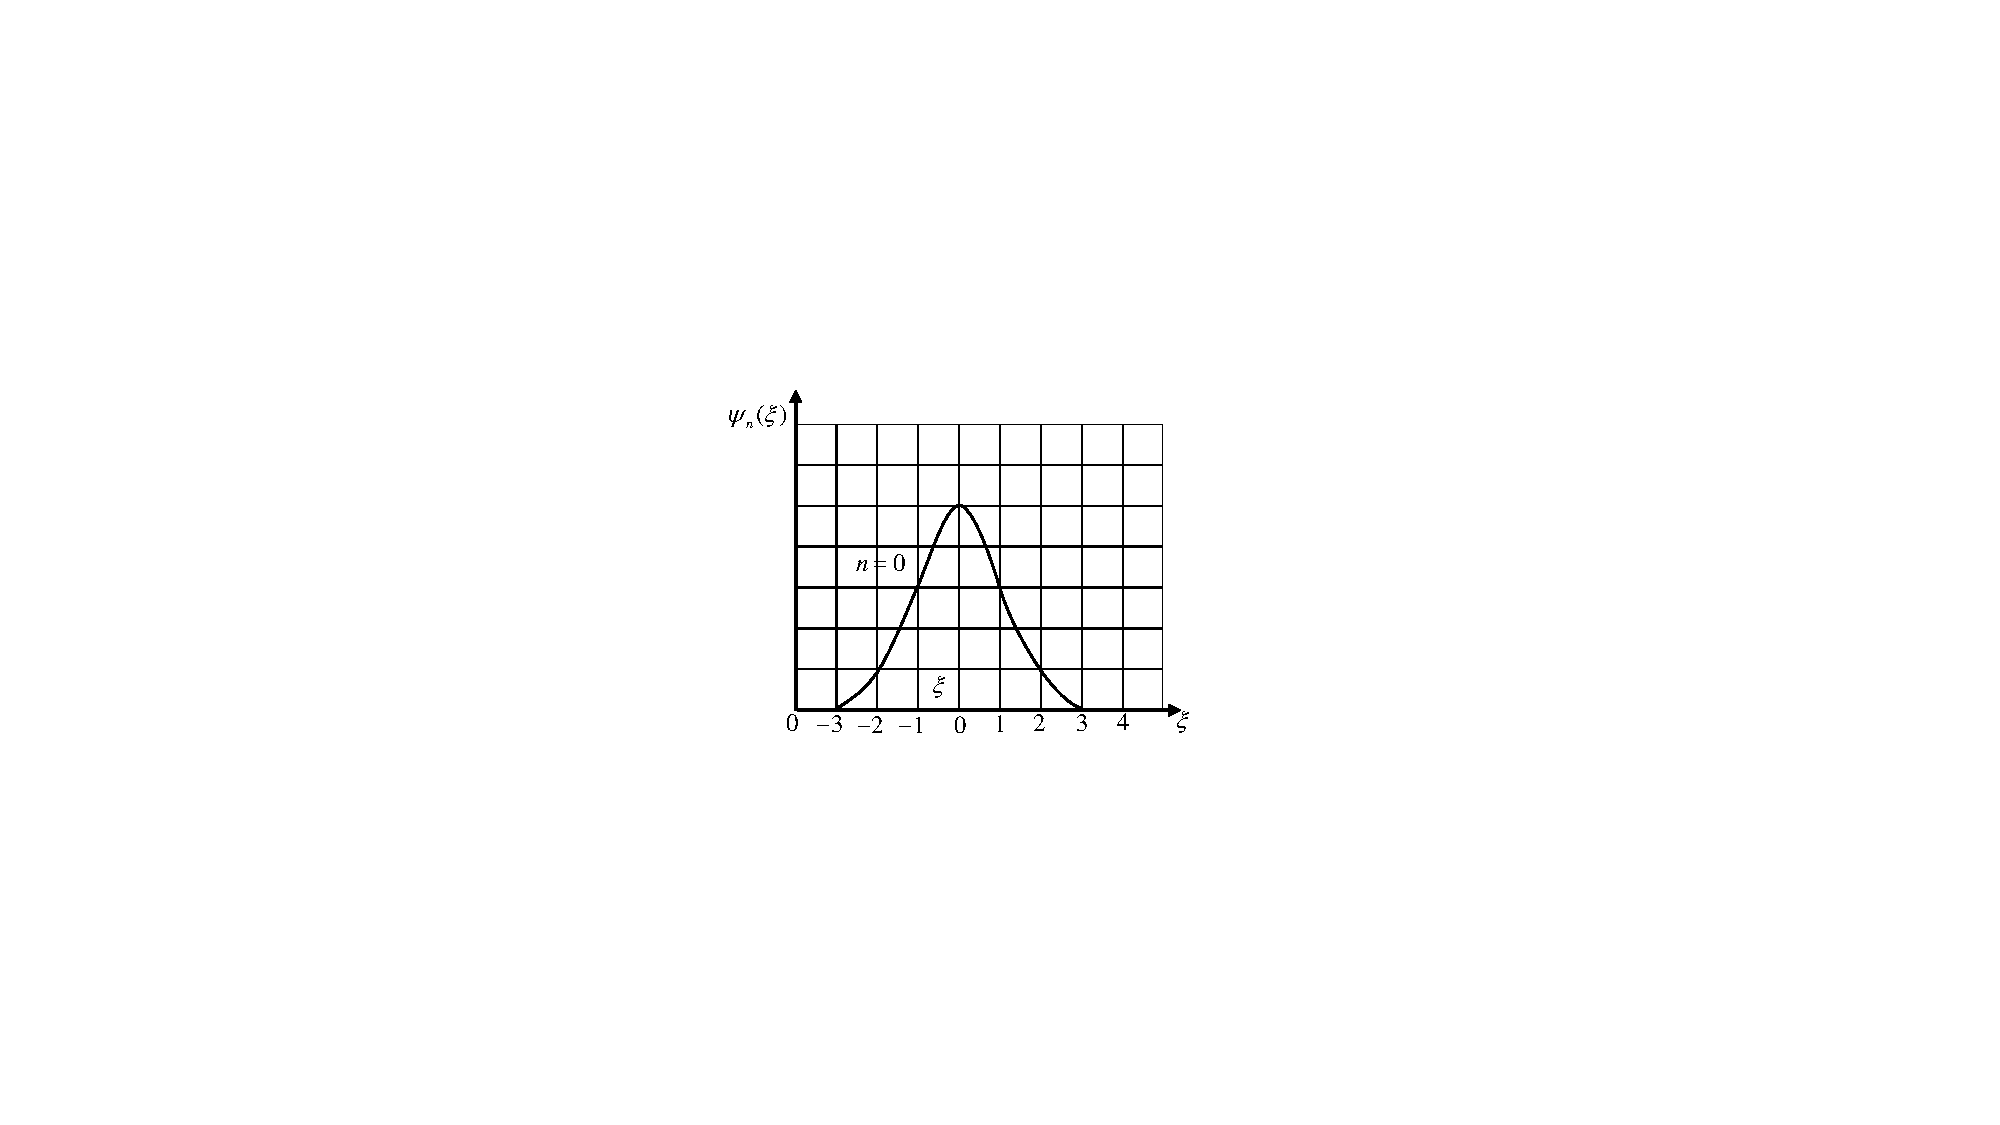
\includegraphics[width=0.6\linewidth]{QM file/figure/2-7(a)}
		%\centerline{(a)}
		\label{fig.2-7(a)}
	\end{minipage}
	\begin{minipage}[h]{0.49\linewidth}
		\centering
		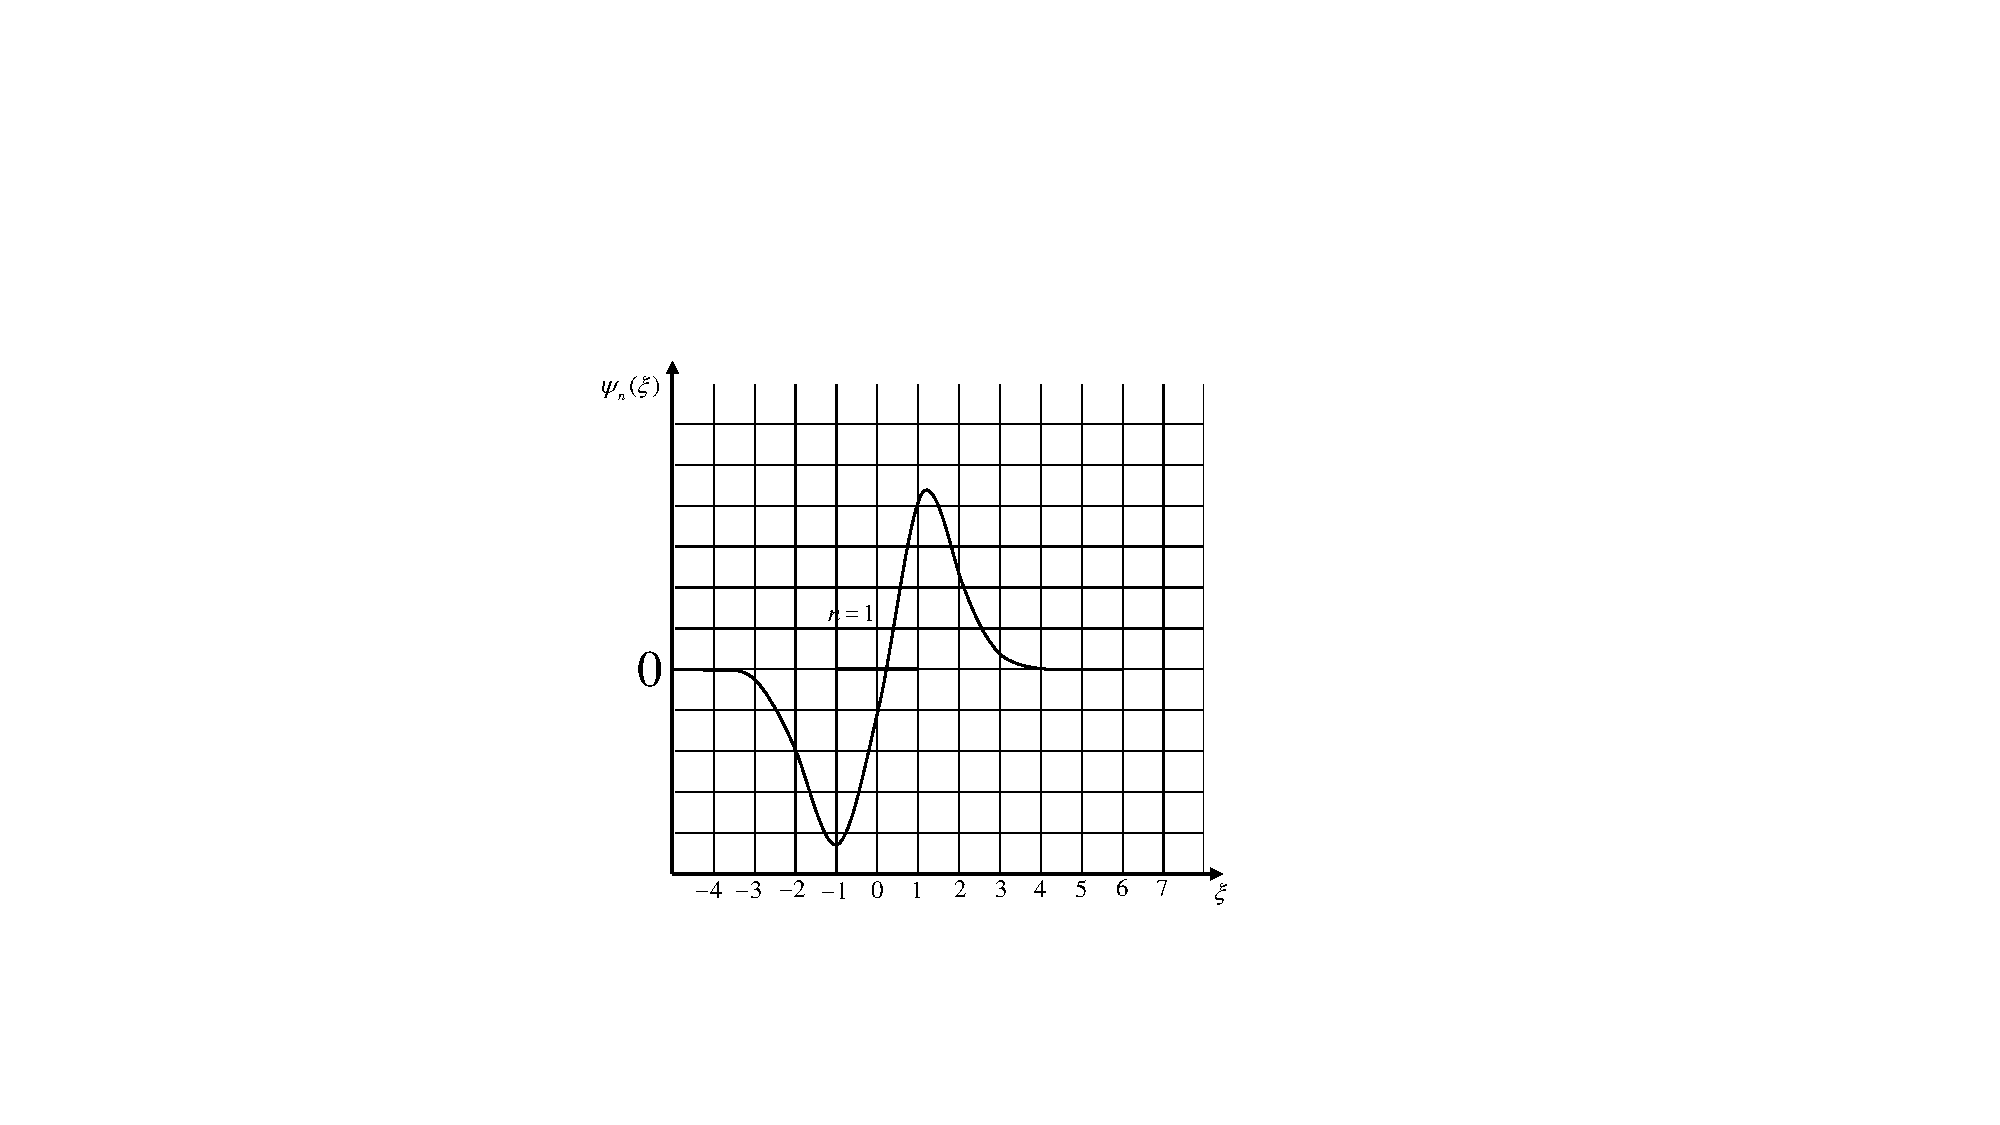
\includegraphics[width=0.6\linewidth]{QM file/figure/2-7(b)}
		%\centerline{(b)}
		\label{fig.2-7(b)}
	\end{minipage}%
	
	\begin{minipage}[h]{0.49\linewidth}
		\centering
		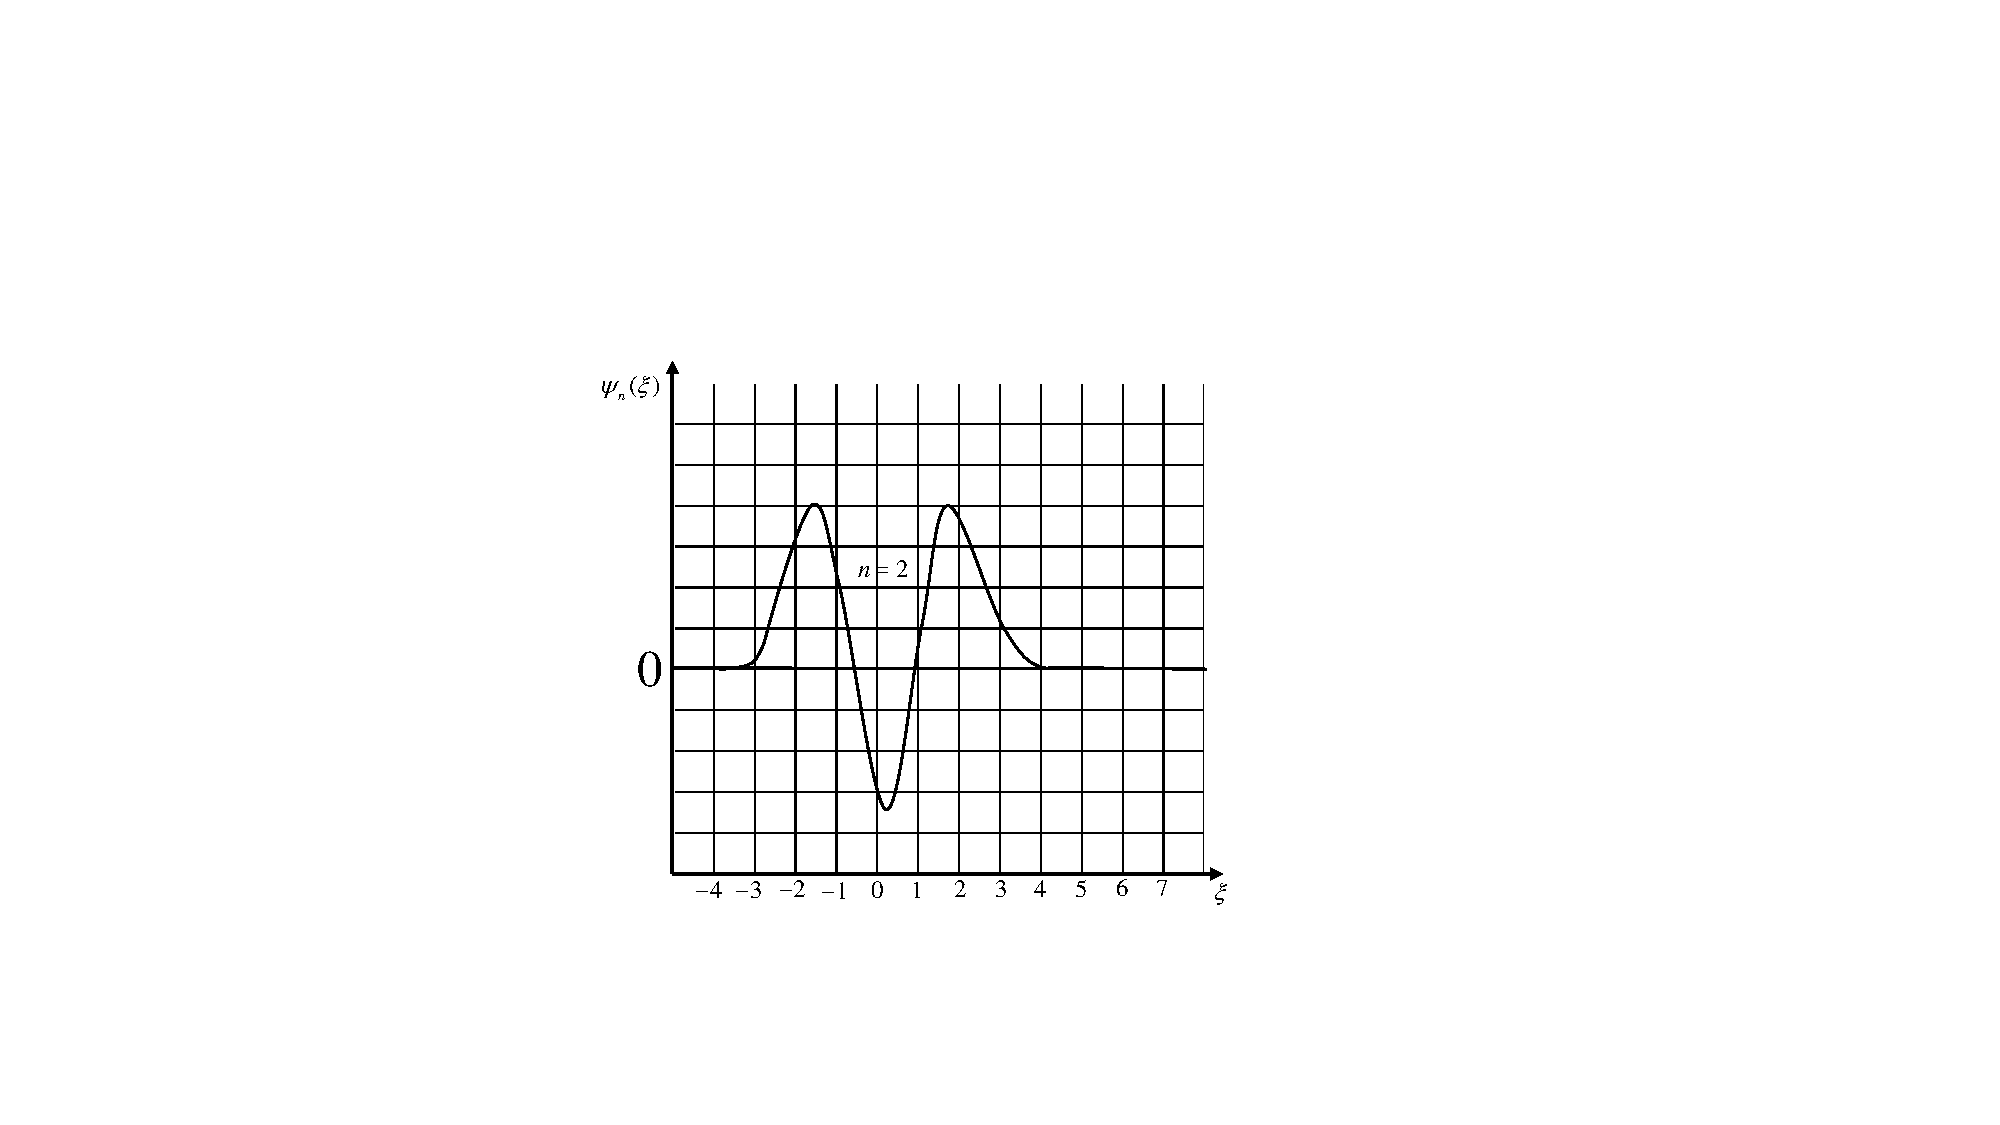
\includegraphics[width=0.6\linewidth]{QM file/figure/2-7(c)}
		%\centerline{(c)}
		\label{fig.2-7(c)}
	\end{minipage}
	\begin{minipage}[h]{0.49\linewidth}
		\centering
		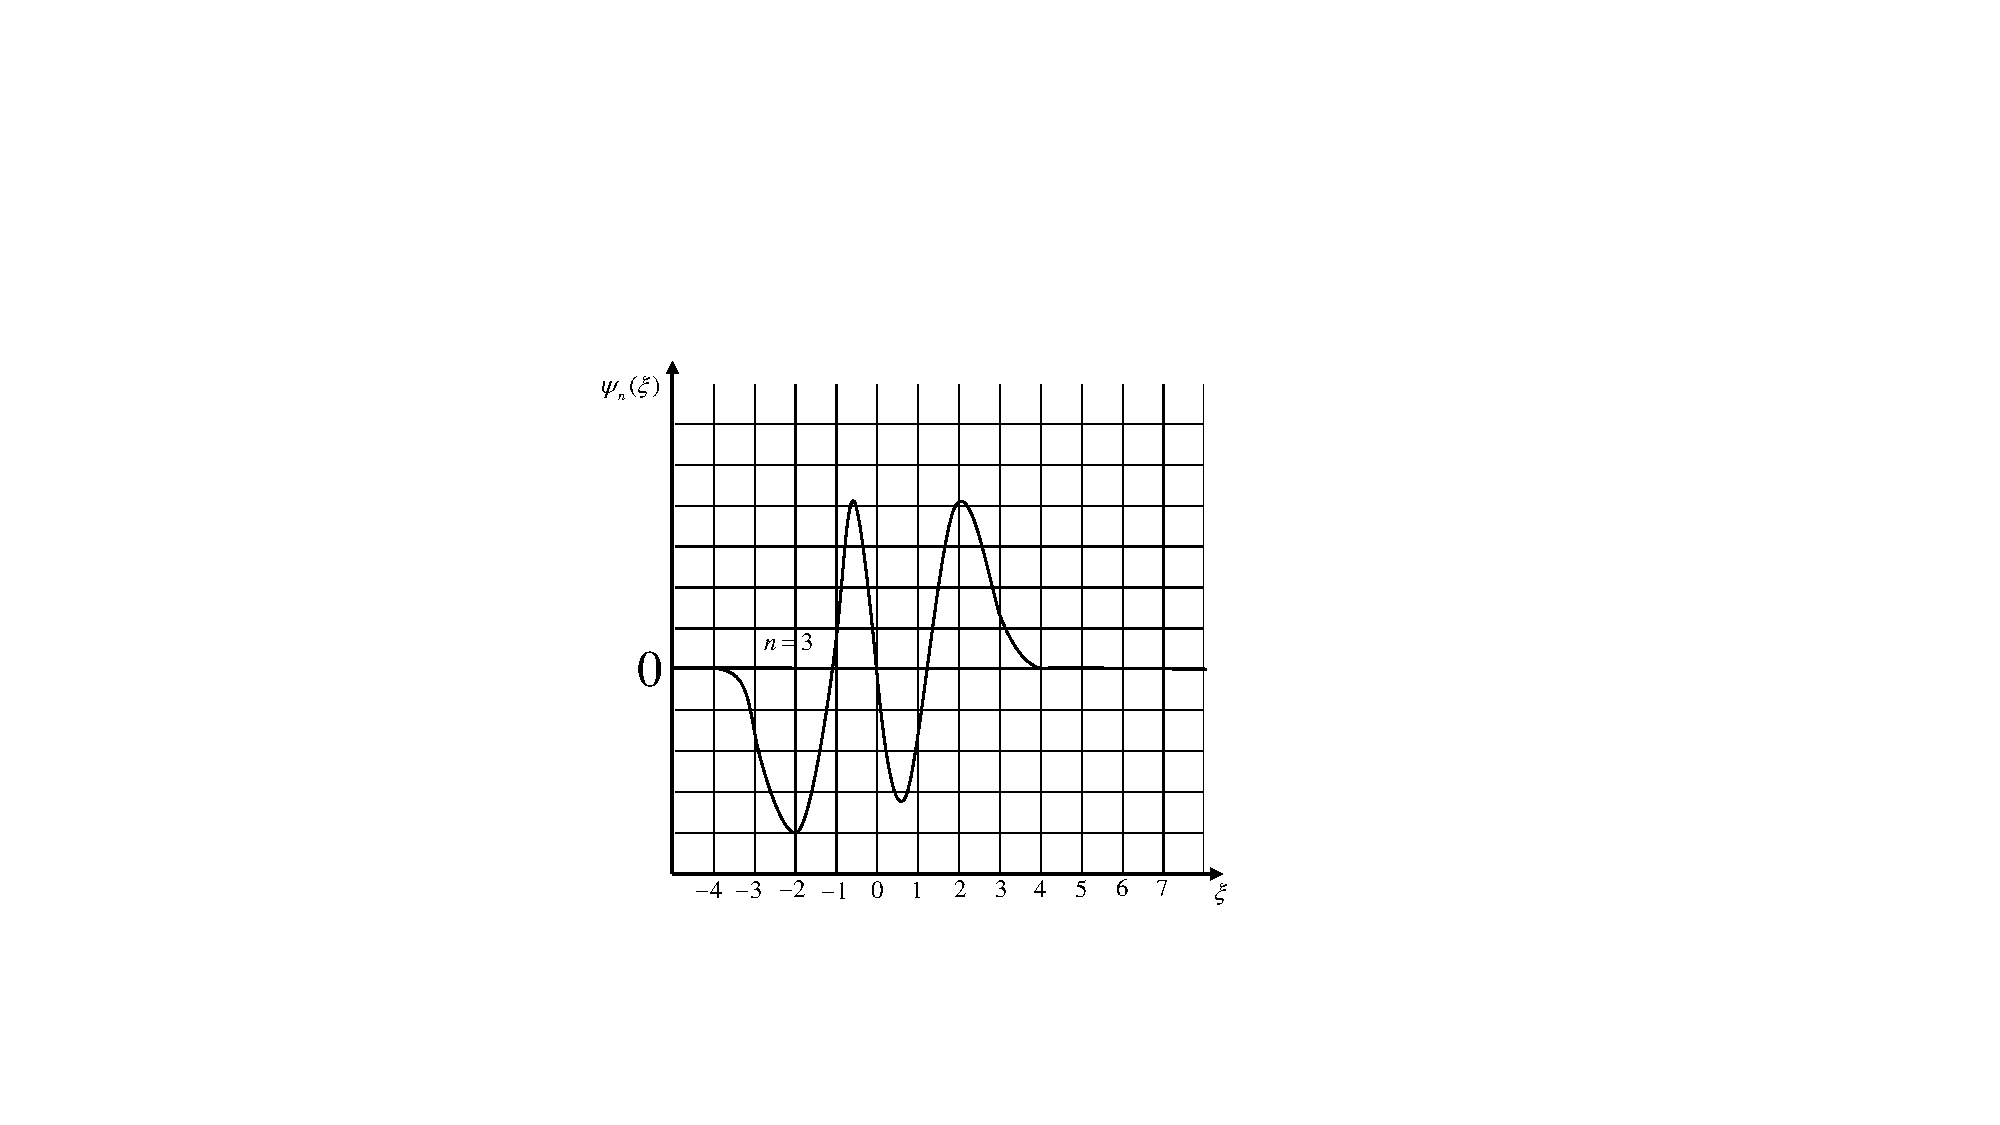
\includegraphics[width=0.6\linewidth]{QM file/figure/2-7(d)}
		%\centerline{(d)}
		\label{fig.2-7(d)}
	\end{minipage}
	\caption{}\label{fig.2-7}
\end{figure}
\begin{empheq}{equation*}
	E=\frac{1}{2}m(\pi v)^{2}A^{2}=2\times 10^{-12} \si{J}
\end{empheq}
而零点能仅为
\begin{empheq}{equation*}
	E_{0}=\frac{\hbar\omega}{2}=\frac{hv}{2}=3.3\times 10^{-34} \si{J}
\end{empheq}
完全不可能测量出来.

按照经典力学,能量为$E$的谐振子,所能达到的离平衡位置($x=0$)最远的距离是$|x|=A=\sqrt{\frac{2E}{m\omega^{2}}}$,$x=\pm A$称为谐振子的经典回转点,按照量子力学,当谐振子处于能量本征态$\varPsi_{n}$时,振子可在也$\varPsi_{n}\neq 0$的一切地点出现.例如,对于基态$\varPsi_{0}$,$E_{0}=\frac{\hbar\omega}{2}$,经典回转点为$|x|=\sqrt{\frac{\hbar}{m\omega}}=x_{0}$,振子在回转点以远(经典禁区)出现概率为
\begin{empheq}{equation}\label{eq25.20}
	2\int_{x_{0}}^{\infty}\varPsi_{0}^{2}dx=\frac{2}{\pi}\int_{1}^{\infty}e^{-\xi^{2}}d\xi=\num{0.1573}
\end{empheq}
对于第一激发态$\varPsi_{1}$,粒子在经典禁区出现的概率为\num{0.1116}.

在经典振幅以内($|x|<A$),量子力学给出的谐振子的空间分布概率也和经典力学结果显然不同.按照量子力学,振子在($x,x+dx$)内出现概率为$|\varPsi(x)|^{2}dx$,呈波浪起伏状.按照经典力学,振子通过($x,x+dx$)区间所用时间为$\frac{dx}{v}$,因此在这区间出现概率为
\setlength{\mathindent}{5em}
\begin{empheq}{equation}\label{eq25.21}
	\frac{\omega dx}{\pi v}=\frac{\omega dx}{\pi\sqrt{\frac{2(E-V)}{m}}}
	=\frac{\sqrt{m}\omega dx}{\pi\sqrt{2E-m\omega^{2}x^{2}}}=\boldsymbol{P}(x)dx
\end{empheq}\eqnormal
$x=0$;$\boldsymbol{P}(x)$为极小;$x\rightarrow\pm A$,$\boldsymbol{P}(x)\rightarrow\infty$.图 \ref{fig.2-8}(a)给出基态$\varPsi_{0}$的量子力学分布概率与经典力学分布概率的对比,两条分布曲线的形状刚好相反.但是,可以证明,当量子数$n$很大时,量子力学概率密度$|\varPsi_{n}(x)|^{2}$的局部平均与经典概率分布$\boldsymbol{P}(x)$趋于一致(对应原理),如图\ref{fig.2-8}(b)所示.
\begin{figure}[!h]
	\centering
		\begin{minipage}{0.49\linewidth}
			\centering
			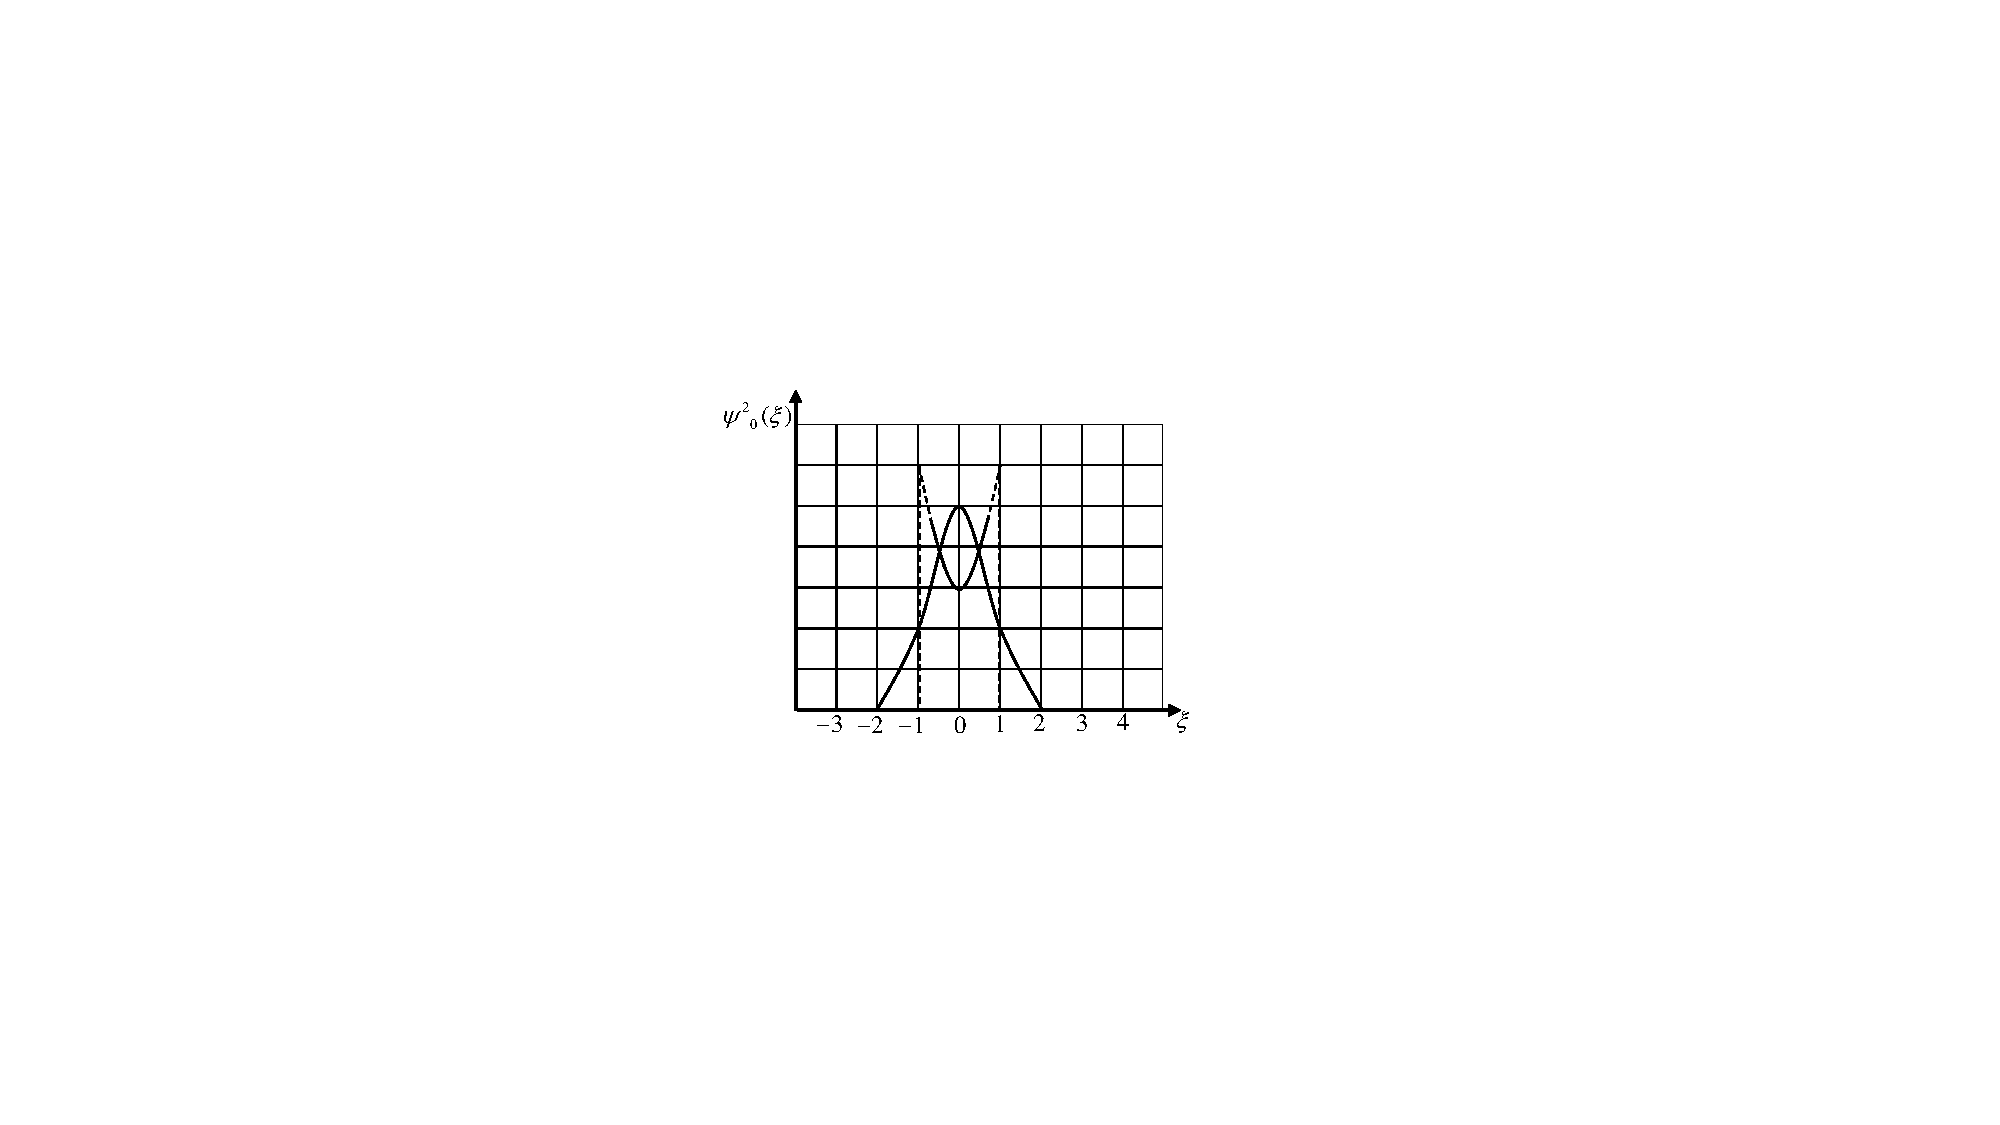
\includegraphics[width=0.7\linewidth]{QM file/figure/2-8(a)}
			\centerline{(a)}
			\label{fig.2-8a}%文中引用该图片代号
		\end{minipage}
		\begin{minipage}{0.49\linewidth}
			\centering
			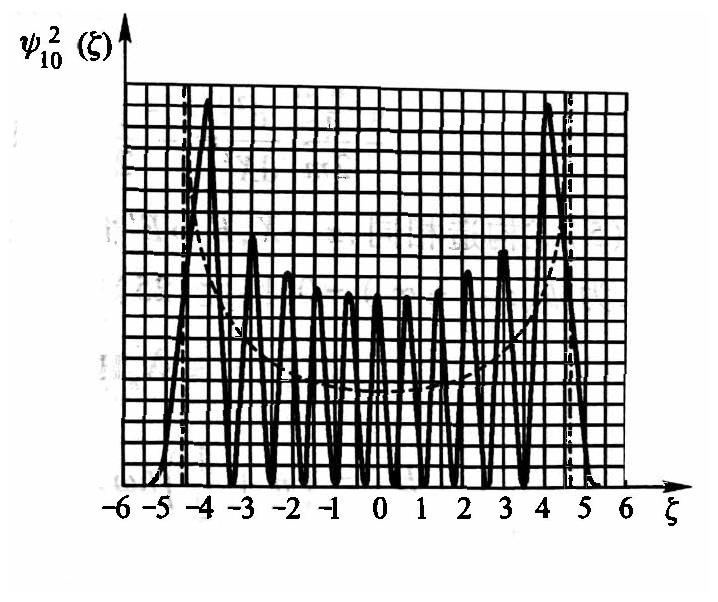
\includegraphics[width=0.7\linewidth]{QM file/figure/2-8(b)}
			\centerline{(b)}
			\label{fig.2-8b}%文中引用该图片代号
		\end{minipage}
	\caption{}\label{fig.2-8}
\end{figure}

图中虚线为经典分布概率曲线.

谐振子的波函数$\varPsi_{n}$相当典型地反映出束缚态波函数的一般特点.在经典允许区($E>V$),$\varPsi^{\prime\prime}$和$\varPsi$异号[参看\eqref{eq25.5}式] ,所以$x-\varPsi$曲线呈波形.在经典回转点,$E=V$,$\varPsi^{\prime\prime}=0$,是$x-\varPsi$曲线的最远的拐点(其他拐点是$\varPsi(x)$的节点).在经典禁区($E<V$),$\varPsi^{\prime\prime}$和$\varPsi$同号,二者随$|x|$的增大而一起衰减为0(波动消失).$\varPsi$开始衰减前的最后一个极大值出现在经典允许区内、经典回转点附近[参看图\ref{fig.2-8}(b)].

\example 质量$m$,电荷$q$的粒子,受到弹性力($-kx$)和均匀电场$\mathscr{E}$(沿正$x$轴方向)的共同作用,势能可以表示为
\begin{empheq}{equation}\label{eq25.22}
	V(x)=\frac{1}{2}kx^{2}-q\mathscr{E}x
\end{empheq}
求定态能级和波函数.

\solution $V(x)$可以表示成下列形式:
\eqlong
\begin{empheq}{equation*}
	V(x)=\frac{k}{2}\bigg(x^{2}-\frac{2q\mathscr{E}}{k}x\bigg)=\frac{k}{2}\bigg(x-\frac{q\mathscr{E}}{k}\bigg)^{2}-\frac{q^{2}\mathscr{E}^{2}}{2k}
\end{empheq}
令$k=m\omega^{2}$,则
\begin{empheq}{equation*}\label{eq25.22'}
	V(x)=\frac{1}{2}m\omega^{2}\bigg(x-\frac{q\mathscr{E}}{m\omega^{2}}\bigg)^{2}-\frac{q^{2}\mathscr{E}^{2}}{2m\omega^{2}}
\end{empheq}
再令
\begin{empheq}{equation}\label{eq25.23}
	X=x-\frac{q\mathscr{E}}{m\omega^{2}},\quad E^{\prime}=E+\frac{q^{2}\mathscr{E}^{2}}{2m\omega^{2}}
\end{empheq}
哈密顿算符可以表示为
\begin{empheq}{equation}\label{eq25.24}
	H=-\frac{\hbar^{2}}{2m}\frac{d^{2}}{dX^{2}}+\frac{1}{2}m\omega^{2}X^{2}-\frac{q^{2}\mathscr{E}^{2}}{2m\omega^{2}}
\end{empheq}
能量本征方程为
\begin{empheq}{equation}\label{eq25.25}
	-\frac{\hbar^{2}}{2m}\frac{d^{2}}{dX^{2}}\varPsi+\frac{1}{2}m\omega^{2}X^{2}\varPsi=E^{\prime}\varPsi
\end{empheq}\eqnormal
\eqref{eq25.25}式与\eqref{eq25.5}式构造相同,$x\rightarrow X$,$E\rightarrow E^{\prime}$而已.无限远处$\varPsi$的边条件也和没有电场时相同,为$\varPsi(x\rightarrow\pm\infty)=0$,因此\eqref{eq25.25}式的特征解必然是
\begin{empheq}{equation}\label{eq25.26}
	\varPsi_{n}(X)=N^{n}H^{n}\bigg(\frac{X}{x_{0}}\bigg)e^{-X^{2}/2x_{0}^{2}}
\end{empheq}
\begin{empheq}{equation}\label{eq25.27}
	E_{n}^{\prime}=\bigg(n+\frac{1}{2}\bigg)\hbar\omega
\end{empheq}
\eqref{eq25.26}式相当于\eqref{eq25.15}式中$x\rightarrow X$.由\eqref{eq25.23}、\eqref{eq25.27}式即得能级为
\eqlong
\begin{empheq}{equation}\label{eq25.28}
	E_{n}=E_{n}^{\prime}-\frac{q^{2}\mathscr{E}^{2}}{2m\omega^{2}}=\bigg(n+\frac{1}{2}\bigg)\hbar\omega-\frac{q^{2}\mathscr{E}}{2m\omega^{2}}
\end{empheq}\eqnormal
总之,电场$E$造成的效果是,各个能级均降低$\frac{q^{2}\mathscr{E}^{2}}{2m\omega^{2}}$,$\varPsi$中$x\rightarrow X$.因此粒子的平衡位置由$x=0$移至$X=0$,即$x=\frac{q\mathscr{E}}{m\omega^{2}}$.亦即粒子的状态向正$x$轴方向平移了距离$\frac{q\mathscr{E}}{m\omega^{2}}$.
